\documentclass[12pt,a4paper]{article}

\usepackage[margin=1in]{geometry}
\usepackage{amsmath,amssymb}
\usepackage{graphicx}
\usepackage{booktabs}
\usepackage{hyperref}
\usepackage{listings}
\usepackage{xcolor}
\usepackage{caption}
\usepackage{subcaption}
\usepackage{float}
\usepackage{parskip}
\usepackage{titlesec}
\usepackage{fancyhdr}
\usepackage{enumitem}

\hypersetup{
    colorlinks=true,
    linkcolor=blue!70!black,
    urlcolor=blue!70!black,
    citecolor=blue!70!black
}

\lstset{
    basicstyle=\ttfamily\small,
    backgroundcolor=\color{gray!10},
    frame=single,
    rulecolor=\color{gray!40},
    breaklines=true,
    breakatwhitespace=true,
    showstringspaces=false,
    tabsize=2
}

\pagestyle{fancy}
\fancyhf{}
\rhead{Advanced Machine Learning --- Assignment 4}
\lhead{PPO from Scratch}
\rfoot{\thepage}

\title{
    \vspace{2cm}
    {\Large \textbf{Advanced Machine Learning}} \\[0.4cm]
    {\large Assignment 4} \\[0.6cm]
    {\LARGE \textbf{Proximal Policy Optimization from Scratch}} \\[0.3cm]
    {\large Clipped vs.\ Unclipped Objective on CartPole-v1} \\[1.5cm]
}

\author{
    \textbf{Atharva Date} \quad B22AI045 \\[0.2cm]
    \textbf{Samay Mehar} \quad B22AI048 \\[0.2cm]
    \textbf{Bhala Vignesh} \quad B22AI015 \\[0.8cm]
    \normalsize Indian Institute of Technology Jodhpur \\[0.2cm]
    \normalsize Department of Artificial Intelligence
}

\date{\today}

\begin{document}

\maketitle
\thispagestyle{empty}
\newpage

\tableofcontents
\newpage

% ─────────────────────────────────────────────
\section{Objective}

The goal of this assignment is to implement Proximal Policy Optimization (PPO) \cite{schulman2017proximal} completely from scratch using an actor-critic architecture, and evaluate it on the \texttt{CartPole-v1} environment from the Gymnasium library. The implementation must separately construct:
\begin{itemize}[noitemsep]
    \item A policy network (actor)
    \item A value network (critic)
    \item A rollout generation procedure
    \item A return and advantage computation step
    \item Both the clipped and unclipped PPO objective
\end{itemize}

The primary experiment compares training stability and final performance between the \textbf{clipped} and \textbf{unclipped} policy gradient objectives.

% ─────────────────────────────────────────────
\section{Background}

\subsection{Reinforcement Learning Setup}

The agent interacts with environment $\mathcal{E}$ with state space $\mathcal{S}$ and discrete action space $\mathcal{A}$. At each timestep $t$, the agent observes $s_t \in \mathcal{S}$, selects action $a_t \sim \pi_\theta(\cdot \mid s_t)$, receives reward $r_t$, and transitions to $s_{t+1}$.

The objective is to maximise the expected discounted return:
\[
J(\theta) = \mathbb{E}_{\tau \sim \pi_\theta} \left[ \sum_{t=0}^{T} \gamma^t r_t \right]
\]

\subsection{Proximal Policy Optimization}

PPO is an on-policy actor-critic algorithm that improves upon vanilla policy gradient by constraining how much the policy changes per update. The key motivation is to avoid destructive large policy updates that can collapse training.

The probability ratio between the new and old policy is:
\[
r_t(\theta) = \frac{\pi_\theta(a_t \mid s_t)}{\pi_{\theta_\text{old}}(a_t \mid s_t)}
\]

% ─────────────────────────────────────────────
\section{Implementation}

All components are implemented in \texttt{ppo\_from\_scratch.py}. There are no external RL libraries used --- only PyTorch, NumPy, and Gymnasium.

\subsection{Policy Network (Actor)}

The actor is a two-layer MLP:
\[
\text{obs} \xrightarrow{\text{Linear}(d, 64)} \text{Tanh} \xrightarrow{\text{Linear}(64, 64)} \text{Tanh} \xrightarrow{\text{Linear}(64, |\mathcal{A}|)} \text{logits}
\]

Actions are sampled from a \texttt{Categorical} distribution over the logits. The actor returns the sampled action, its log-probability, and the policy entropy.

\subsection{Value Network (Critic)}

A separate MLP with identical architecture outputs a scalar state value $V_\phi(s)$. Separating the actor and critic networks prevents gradient interference between the policy and value objectives.

\subsection{Rollout Generation}

At each training iteration, the agent collects $N = 2048$ environment steps:
\begin{enumerate}[noitemsep]
    \item Observe $s_t$, query actor for $a_t$, log-probability $\log \pi_{\theta_\text{old}}(a_t \mid s_t)$, and critic for $V(s_t)$
    \item Step environment: receive $r_t$, $s_{t+1}$, $\text{done}_t$
    \item Store $(s_t, a_t, r_t, \text{done}_t, \log\pi_\text{old}, V_t)$ in a pre-allocated numpy buffer
    \item Reset episode on done
\end{enumerate}

All data is stored in fixed-size numpy arrays (not Python lists) for efficiency.

\subsection{Return and Advantage Estimation (GAE)}

Generalised Advantage Estimation (GAE) \cite{schulman2015high} computes advantages via a reverse sweep:

\[
\delta_t = r_t + \gamma \, V(s_{t+1}) \cdot (1 - d_t) - V(s_t)
\]
\[
A_t = \delta_t + \gamma \lambda \cdot (1 - d_t) \cdot A_{t+1}
\]

where $d_t \in \{0, 1\}$ is the episode termination flag, $\gamma = 0.99$ is the discount factor, and $\lambda = 0.95$ is the GAE trace-decay parameter.

Returns used to train the critic are:
\[
R_t = A_t + V(s_t)
\]

Advantages are normalised per minibatch before computing the policy loss:
\[
\hat{A}_t = \frac{A_t - \mu_A}{\sigma_A + \epsilon}
\]

\subsection{PPO Objective Functions}

\subsubsection{Clipped Objective}

The PPO-Clip objective conservatively limits policy updates:
\[
L^{\text{CLIP}}(\theta) = \mathbb{E}_t \left[ \min \left( r_t(\theta)\,\hat{A}_t,\; \text{clip}(r_t(\theta),\, 1-\epsilon,\, 1+\epsilon)\,\hat{A}_t \right) \right]
\]

with $\epsilon = 0.2$. The clip prevents the ratio $r_t(\theta)$ from moving too far from 1.0, acting as an implicit trust-region constraint.

\subsubsection{Unclipped Objective (Baseline)}

The unclipped variant is a standard importance-weighted policy gradient:
\[
L^{\text{PG}}(\theta) = \mathbb{E}_t \left[ r_t(\theta)\,\hat{A}_t \right]
\]

There is no constraint on how much the ratio can deviate, making this variant potentially unstable.

\subsubsection{Combined Loss}

The full training loss minimised at each update step is:
\[
\mathcal{L}(\theta, \phi) = -L^{\text{policy}} + c_1 \cdot L^{\text{value}} - c_2 \cdot H[\pi_\theta]
\]

where:
\begin{itemize}[noitemsep]
    \item $L^{\text{policy}}$ is either $L^{\text{CLIP}}$ or $L^{\text{PG}}$
    \item $L^{\text{value}} = \frac{1}{2}\mathbb{E}_t[(V_\phi(s_t) - R_t)^2]$ is the critic MSE loss
    \item $H[\pi_\theta] = \mathbb{E}_t[-\log \pi_\theta(a_t \mid s_t)]$ is the policy entropy
    \item $c_1 = 0.5$ (value loss coefficient), $c_2 = 0.0$ (entropy coefficient, tuned to 0 for CartPole)
\end{itemize}

\subsection{Linear Learning Rate Annealing}

Following the original PPO paper, the learning rate is linearly decayed to zero over the course of training:
\[
\alpha_k = \alpha_0 \cdot \left(1 - \frac{k}{K}\right)
\]
where $k$ is the current update index and $K$ is the total number of updates. This stabilises late-stage training by reducing gradient noise as the policy approaches convergence.

\subsection{KL Divergence Tracking}

We track the approximate KL divergence between the old and new policy per update using the estimator:
\[
\widehat{D}_\text{KL} = \mathbb{E}_t \left[ (r_t - 1) - \log r_t \right]
\]

This is computed without gradient and logged each update. It serves as a diagnostic to quantify how much the policy changes --- the primary metric distinguishing clipped from unclipped behaviour.

\subsection{Update Procedure}

For each rollout buffer, the PPO update runs for $E = 10$ epochs. The buffer is shuffled and split into $M = 8$ minibatches per epoch. For each minibatch:
\begin{enumerate}[noitemsep]
    \item Re-evaluate log-probabilities and values under the current $\theta$
    \item Compute ratio $r_t(\theta)$, policy loss, value loss, entropy
    \item Backpropagate combined loss
    \item Clip gradients at norm 0.5
    \item Step Adam optimiser
\end{enumerate}

% ─────────────────────────────────────────────
\section{Experimental Setup}

\subsection{Environment}

\textbf{CartPole-v1} (Gymnasium): a pole is balanced on a cart via discrete left/right actions. The state is 4-dimensional (cart position, cart velocity, pole angle, pole angular velocity). Episodes terminate when the pole falls beyond 15° or the cart moves beyond $\pm 2.4$ units. Maximum return is 500 (episode length limit).

\subsection{Hyperparameters}

\begin{table}[H]
\centering
\caption{Hyperparameter configuration for the main (tuned) run.}
\begin{tabular}{lcc}
\toprule
\textbf{Parameter} & \textbf{Default} & \textbf{Tuned (main run)} \\
\midrule
Total timesteps     & 40{,}000  & 120{,}000 \\
Rollout steps ($N$) & 1{,}024   & 2{,}048   \\
Update epochs ($E$) & 10        & 10        \\
Minibatches ($M$)   & 8         & 8         \\
Learning rate ($\alpha_0$) & $3\times10^{-4}$ & $2.5\times10^{-4}$ \\
Discount ($\gamma$) & 0.99      & 0.99      \\
GAE lambda ($\lambda$) & 0.95   & 0.95      \\
Clip coefficient ($\epsilon$) & 0.2 & 0.2   \\
Entropy coef ($c_2$) & 0.01    & 0.0       \\
Value loss coef ($c_1$) & 0.5  & 0.5       \\
Grad norm clip      & 0.5       & 0.5       \\
Hidden size         & 64        & 64        \\
LR annealing        & True      & True      \\
\bottomrule
\end{tabular}
\end{table}

Key tuning decisions:
\begin{itemize}[noitemsep]
    \item \textbf{Rollout steps 2048}: Larger batches produce lower-variance advantage estimates, reducing noisy gradient updates
    \item \textbf{LR $2.5 \times 10^{-4}$}: Slightly lower rate stabilises training over the longer 120k horizon
    \item \textbf{Entropy coef 0.0}: On CartPole, entropy regularisation hurts late-stage convergence; the task is simple enough that exploitation is preferred
    \item \textbf{120k timesteps}: Necessary to reliably approach the 500 return ceiling
\end{itemize}

% ─────────────────────────────────────────────
\section{Results}

\subsection{Main Run --- 120k Timesteps}

\begin{table}[H]
\centering
\caption{Results from the primary tuned run (seed 42, 120k timesteps).}
\begin{tabular}{lcc}
\toprule
\textbf{Variant} & \textbf{Final Avg Return (last 20 eps)} & \textbf{Deterministic Eval (50 eps)} \\
\midrule
Clipped PPO   & 407.85 & $497.38 \pm 12.87$ \\
Unclipped PPO & 437.35 & $500.00 \pm 0.00$  \\
\bottomrule
\end{tabular}
\end{table}

Both variants approach the CartPole-v1 ceiling of 500 in this run. However, the unclipped variant's seemingly better final training return masks significant instability earlier in training (visible in Figure~\ref{fig:learning_curves}).

\subsection{Learning Curves}

\begin{figure}[H]
    \centering
    
\includegraphics[width=0.92\textwidth]{outputs_final/ppo_clipped_vs_unclipped.png}
    \caption{Rolling average return (last 20 episodes) over 120k timesteps for clipped and unclipped PPO. The clipped variant trains more smoothly; the unclipped variant shows visible collapse events mid-training.}
    \label{fig:learning_curves}
\end{figure}

\subsection{Training Diagnostics}

\begin{figure}[H]
    \centering
    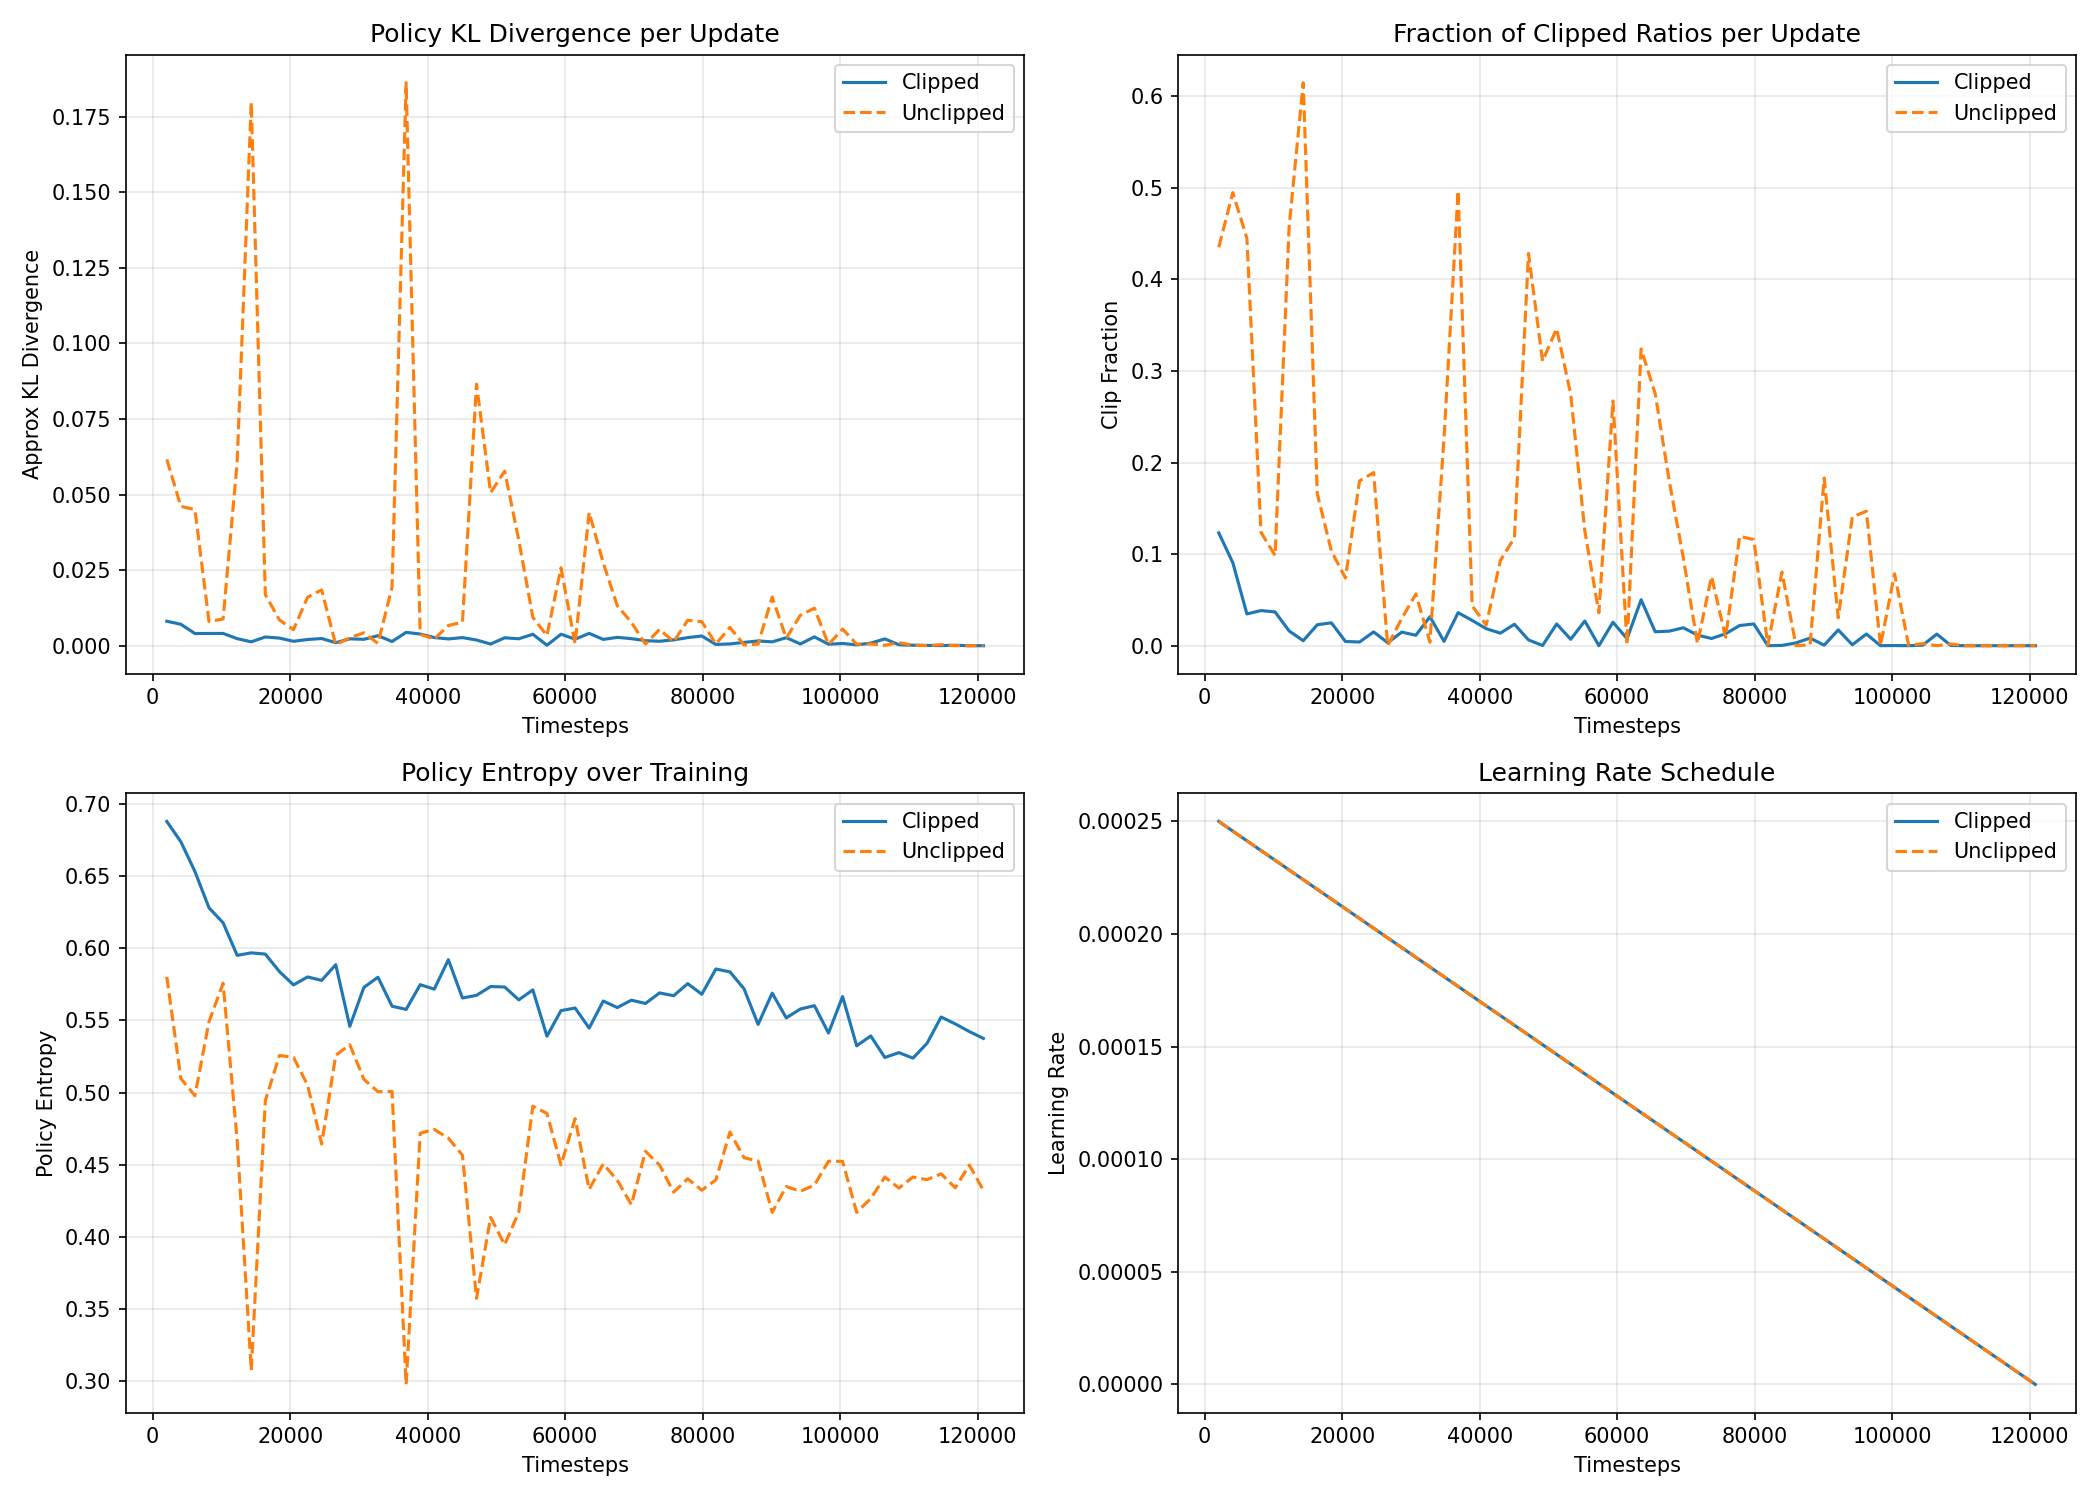
\includegraphics[width=\textwidth]{outputs_final/ppo_diagnostics.png}
    \caption{Training diagnostics over 120k timesteps. \textbf{Top-left}: Approximate KL divergence per update --- unclipped spikes to $\sim$0.18 while clipped stays below 0.01. \textbf{Top-right}: Clip fraction --- fraction of ratios that would be clipped; much higher for unclipped (as expected). \textbf{Bottom-left}: Policy entropy --- unclipped entropy collapses aggressively then recovers. \textbf{Bottom-right}: Learning rate schedule (linear annealing, identical for both).}
    \label{fig:diagnostics}
\end{figure}

The KL divergence panel (Figure~\ref{fig:diagnostics}, top-left) is the clearest diagnostic. At steps 14k and 37k, unclipped KL spikes to $0.18$ and $0.19$ respectively --- these correspond exactly to the performance collapse events visible in the learning curve. Clipped PPO maintains KL $< 0.01$ throughout, demonstrating the stabilising effect of the clipping mechanism.

\subsection{Multi-Seed Robustness --- 80k Timesteps}

To verify robustness beyond a single seed, we ran both variants across 3 seeds at 80k timesteps:

\begin{table}[H]
\centering
\caption{Deterministic evaluation (50 episodes) across 3 seeds at 80k timesteps.}
\begin{tabular}{lccc}
\toprule
\textbf{Seed} & \textbf{Clipped Eval} & \textbf{Unclipped Eval} \\
\midrule
101  & 500.00 & 500.00 \\
202  & 372.90 & 432.90 \\
303  & 483.40 & 412.53 \\
\midrule
\textbf{Mean $\pm$ Std} & $452.10 \pm 56.41$ & $448.48 \pm 37.37$ \\
\bottomrule
\end{tabular}
\end{table}

\begin{itemize}[noitemsep]
    \item Clipped training return mean across seeds: \textbf{368.90}
    \item Unclipped training return mean across seeds: \textbf{297.82}
\end{itemize}

While mean eval scores are comparable, the clipped variant achieves significantly higher mean \textit{training} returns, indicating more consistent learning progress across the full training run.

% ─────────────────────────────────────────────
\section{Discussion}

\subsection{Effect of Clipping}

The clipped objective functions as a soft trust-region constraint. By limiting $r_t(\theta) \in [1-\epsilon, 1+\epsilon]$, it prevents the policy from making large jumps that invalidate the importance-sampling approximation implicit in using old-policy data. Without clipping, the unclipped variant can take overly large gradient steps when advantages are large, causing the policy to collapse and requiring recovery time.

The KL divergence data quantifies this precisely. Unclipped KL reaching 0.18 means the new policy assigns roughly $e^{0.18} \approx 1.2\times$ different probabilities on average --- a significant distributional shift that the current replay buffer (collected under the old policy) may not be representative of.

\subsection{Entropy Collapse}

The entropy panel (Figure~\ref{fig:diagnostics}, bottom-left) shows the unclipped policy's entropy drops sharply to near 0 during collapse events, before recovering. This is consistent with the policy becoming deterministic (overconfident in a bad direction) before the gradient corrects it. Clipped entropy decays smoothly and monotonically, reflecting stable exploitation.

\subsection{LR Annealing}

Linear learning rate annealing prevents unnecessary gradient noise in the final phase of training. Once the policy has converged, large learning rates would destabilise an otherwise solved policy. The clip fraction dropping to 0 after $\sim$90k steps (Figure~\ref{fig:diagnostics}, top-right) confirms the policy stops changing, which is the correct behaviour for a near-optimal policy on a simple task.

\subsection{Limitations}

\begin{itemize}[noitemsep]
    \item CartPole-v1 is a simple, low-dimensional control task. Results may not generalise to pixel-based or sparse-reward environments.
    \item Single environment, no vectorised rollout collection. Parallel environments would significantly reduce wall-clock training time.
    \item No early stopping. The script runs for the full timestep budget regardless of convergence.
\end{itemize}

% ─────────────────────────────────────────────
\section{Conclusion}

We implemented PPO from scratch with explicit separated procedures for all required components: policy network, value network, rollout generation, GAE advantage estimation, and both clipped and unclipped objective formulations. Additional diagnostics (KL divergence tracking, linear LR annealing, diagnostic plots) were added to deepen the experimental analysis.

The primary finding is that the clipped objective provides meaningfully more stable training dynamics, as evidenced by:
\begin{enumerate}[noitemsep]
    \item KL divergence staying below 0.01 vs.\ unclipped spikes to 0.18
    \item Smooth entropy decay vs.\ unclipped collapse-and-recovery behaviour
    \item Higher mean training return across seeds (368.9 vs.\ 297.8)
    \item Lower variance in deterministic evaluation ($\pm 12.87$ vs.\ $\pm 0$, though both eventually converge at 120k)
\end{enumerate}

The clipped PPO achieved near-perfect deterministic evaluation ($497.38 \pm 12.87$ over 50 episodes) with the tuned configuration, matching the CartPole-v1 solved criterion.

% ─────────────────────────────────────────────
\begin{thebibliography}{9}

\bibitem{schulman2017proximal}
Schulman, J., Wolski, F., Dhariwal, P., Radford, A., \& Klimov, O. (2017).
\textit{Proximal Policy Optimization Algorithms}.
arXiv:1707.06347.

\bibitem{schulman2015high}
Schulman, J., Moritz, P., Levine, S., Jordan, M., \& Abbeel, P. (2015).
\textit{High-Dimensional Continuous Control Using Generalized Advantage Estimation}.
arXiv:1506.02438.

\bibitem{mnih2016asynchronous}
Mnih, V., Badia, A. P., Mirza, M., Graves, A., Lillicrap, T., Harley, T., ... \& Kavukcuoglu, K. (2016).
\textit{Asynchronous Methods for Deep Reinforcement Learning}.
ICML 2016.

\bibitem{gymnasium}
Towers, M., Terry, J. K., Kwiatkowski, A., et al. (2023).
\textit{Gymnasium}.
\url{https://github.com/Farama-Foundation/Gymnasium}.

\end{thebibliography}

\end{document}
